\documentclass[noback,noborder,portrait,twocolumn]{cuposter}

%%\documentclass[noback,portrait]{cuposter}
%% To make a poster in portrait, use the "portrait" option to
%% documentclass as shown above.

\usepackage{mathptmx}
\usepackage{xspace}
\usepackage{amsmath}
\usepackage{pifont}
\usepackage{psfrag}

\usepackage{graphicx}
%% \usepackage{subcaption}
\usepackage{wrapfig}
\usepackage{../macros}



\begin{document}

%% Not needed for most posters.
%%\renewcommand{\poster@ancimage}{/tmp/empty.ps}
%% \newcommand{\don}{\ensuremath{d_{\textsc{ON}}}}
%% \newcommand{\doff}{\ensuremath{d_{\textsc{OFF}}}}
%% \newcommand{\dsoma}{\ensuremath{d_{\textsc{SOMA}}} \xspace}
%% \newcommand{\um}{\ensuremath{\mu \text{m}}\xspace}
%% \newcommand{\dmin}{d$_{\textup{min}}$\xspace}

\newcommand{\figspace}{\vskip 20pt plus 5pt minus 5pt}
\newcommand{\captionspace}{\vskip 10pt plus 5pt minus 5pt}

%%%NOTE: \linewidth IS THE CORRECT MACRO FOR SPECIFYING THE LENGTH OF COLUMNS

\newcounter{figcounter}
\newcommand{\getIncFigcounter}{\stepcounter{figcounter}\thefigcounter}
\title{\sciwms{}: Python Based Web Mapping Service For Visualizing Geospatial Data}

\newcounter{tablecounter}
\newcommand{\getIncTablecounter}{\stepcounter{tablecounter}\thetablecounter}

%%\subtitle{The poster subtitle here}
\author{Brandon A. Mayer$^{1,2}$, Brian McKenna$^{2}$, Dave A. Foster$^{2}$, Kelly Knee$^{2}$}
\address{Brown University, Providence RI, USA$^{1}$; RPS-ASA, South Kingston RI, USA$^{2}$}
%% \address{$^1$University of Cambridge and University of Edinburgh, UK;
%%   $^2$University of Lancaster, UK; $^3$Northwestern University, USA.}

\makeposter

\section{Introduction}
\sciwms{} is an open-source python implementation of the \ogc{} \wms{} service for qualitatively assessing society-critical atmostpheric and oceanagraphic model and forcasting data including:

\begin{itemize}
  \item forecasting
  \item risk assessment
  \item model comparison
  \item algorithmic/parameter selection
\end{itemize}

\sciwms{} source code is available at https://github.com/brandonmayer/sci-wms/tree/testbed

\begin{minipage}[r]{\linewidth}
  \centering
  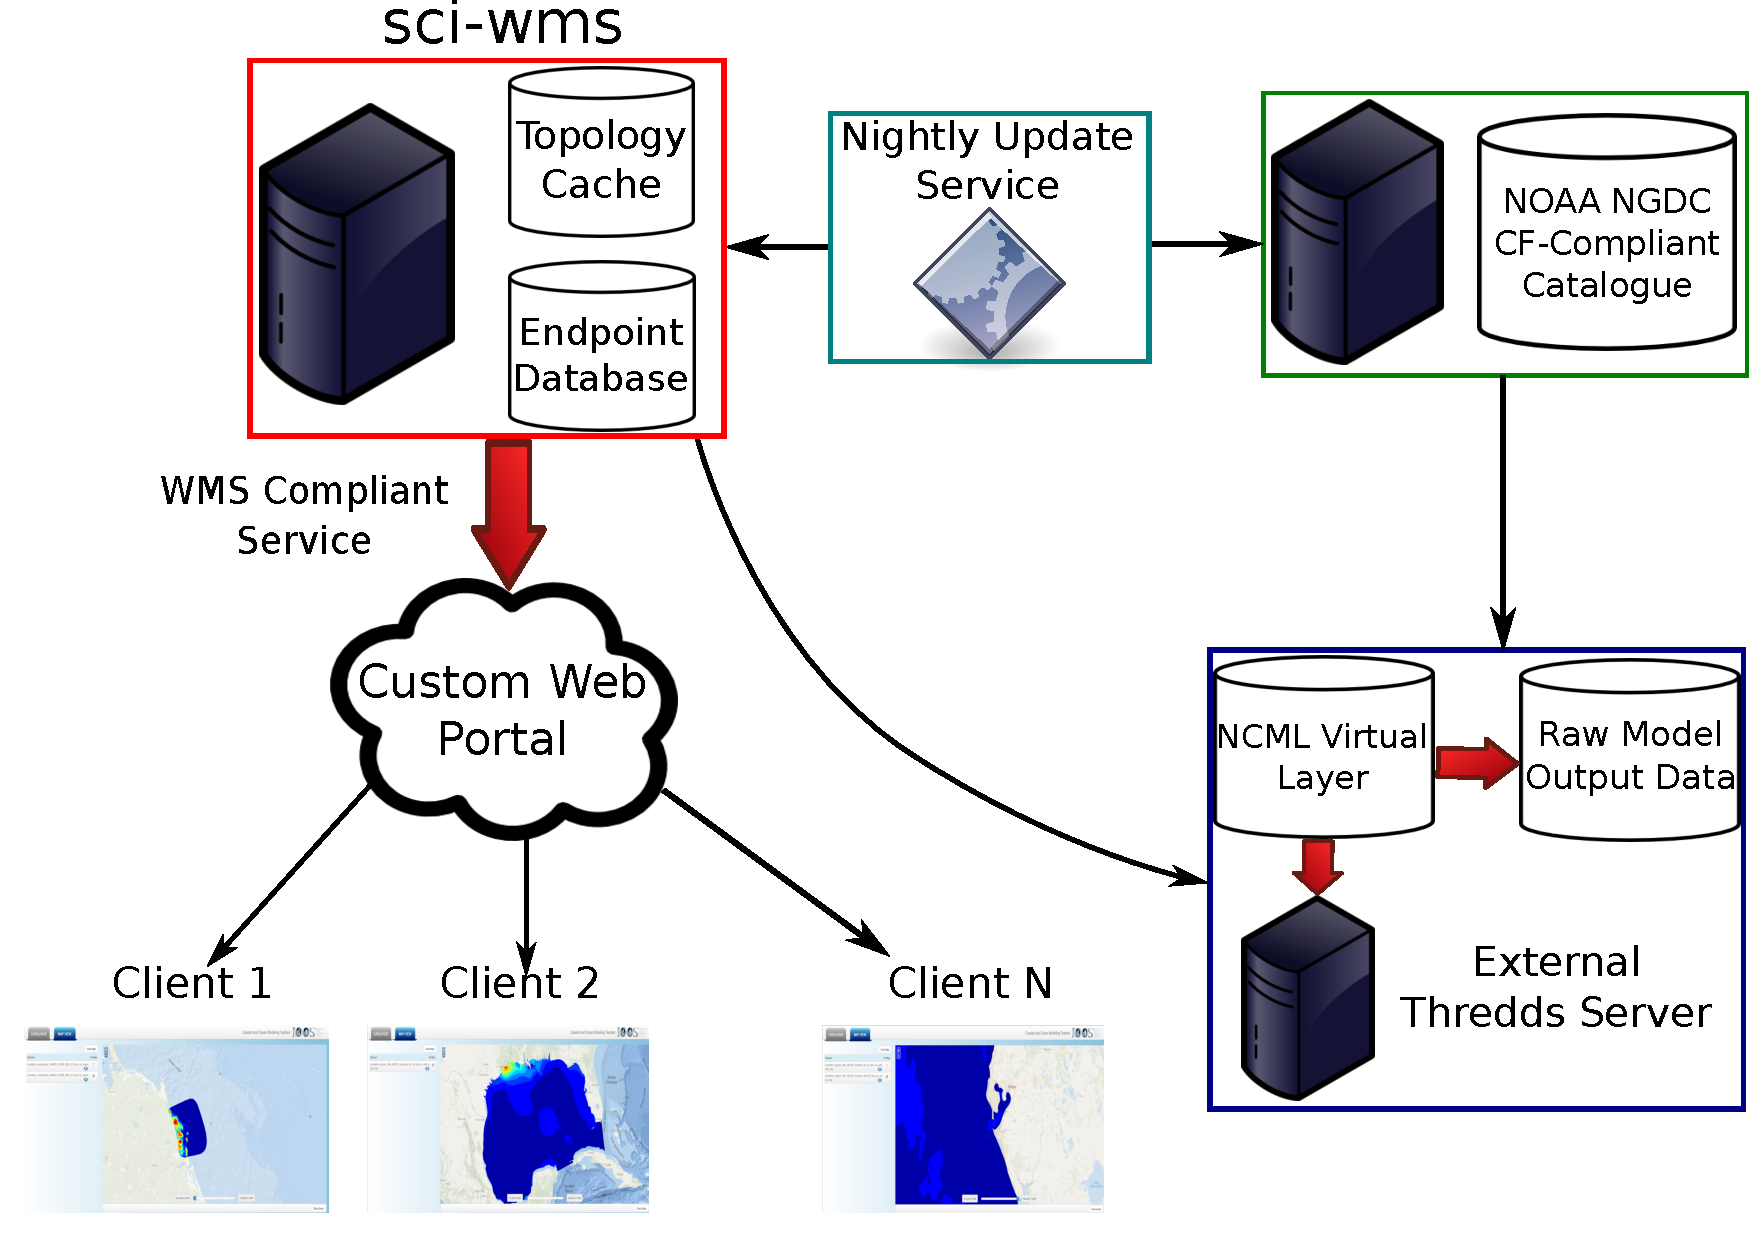
\includegraphics[width=\linewidth]{../figs/overview.pdf}
  \captionspace{}
  \textbf{Figure \getIncFigcounter{}}: \textit{Overview of the \sciwms{} architecture within the scope of the U.S. \ioos{} \comt{} project.}
\end{minipage}

\begin{minipage}[t]{\linewidth}
  \centering
  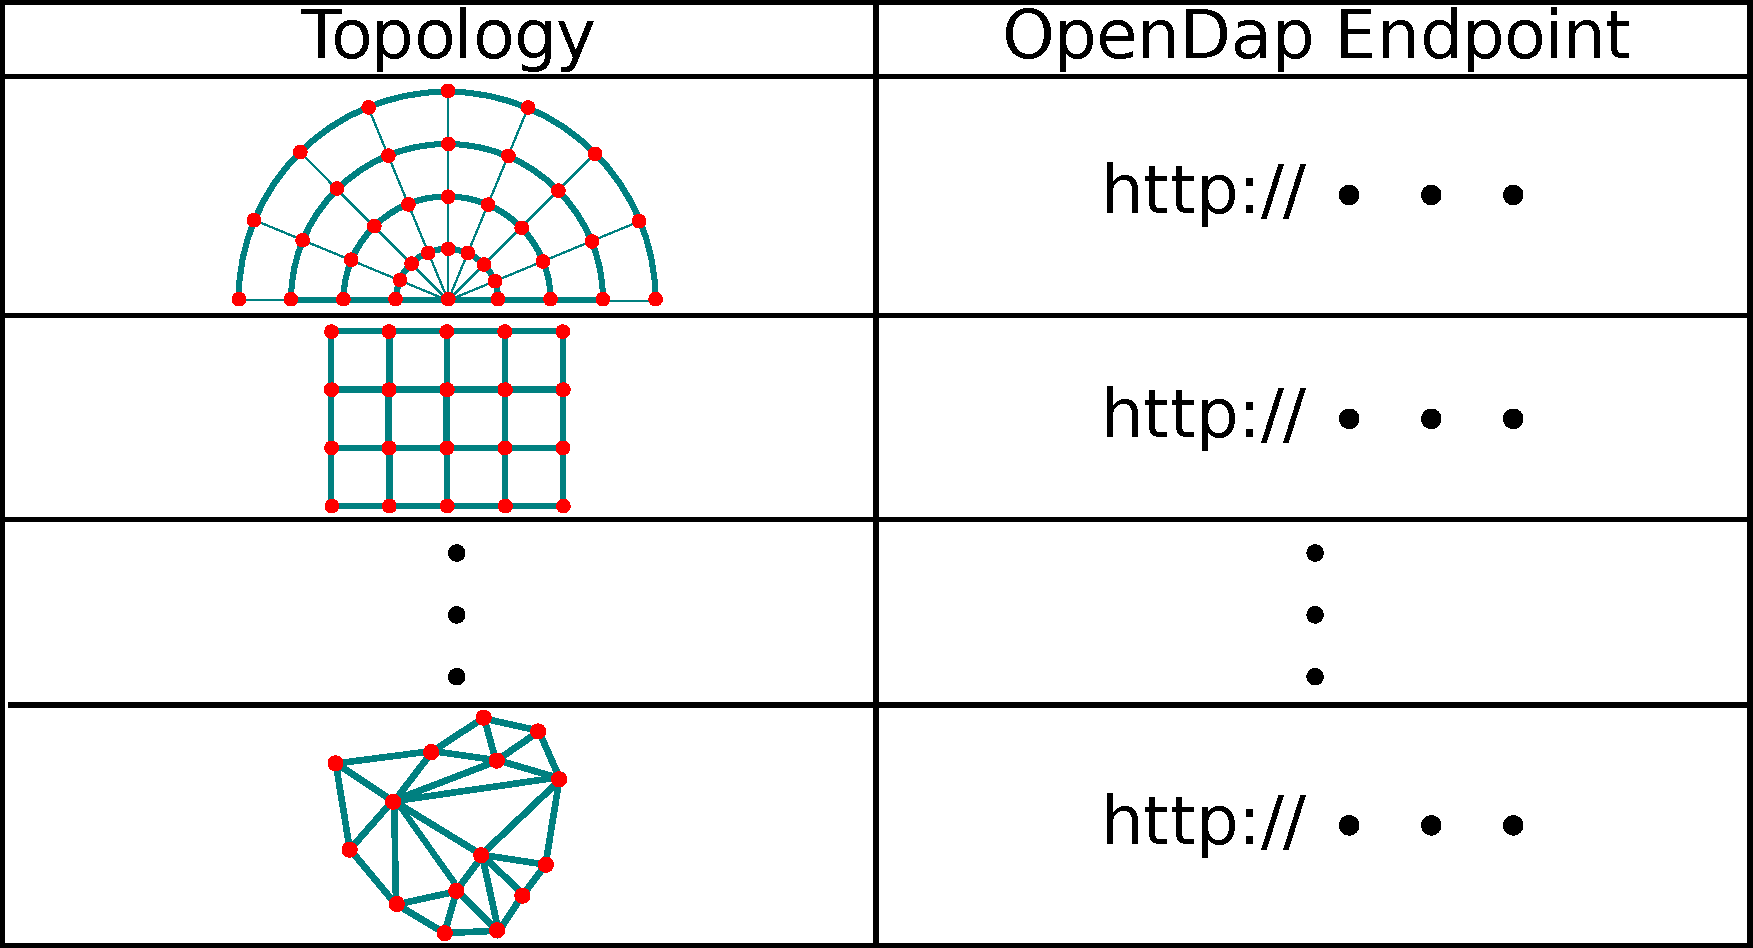
\includegraphics[width=\linewidth]{../figs/sciwms_db_topology_endpoints.pdf}
  \textbf{Figure \getIncFigcounter{}}: \textit{Topology and endpoint data store. Topologies are classified as either \cgrid{} or \ugrid{} for efficient geospatial queries and remote model data access.}
\end{minipage}

\begin{minipage}[t]{\linewidth}
  \centering
  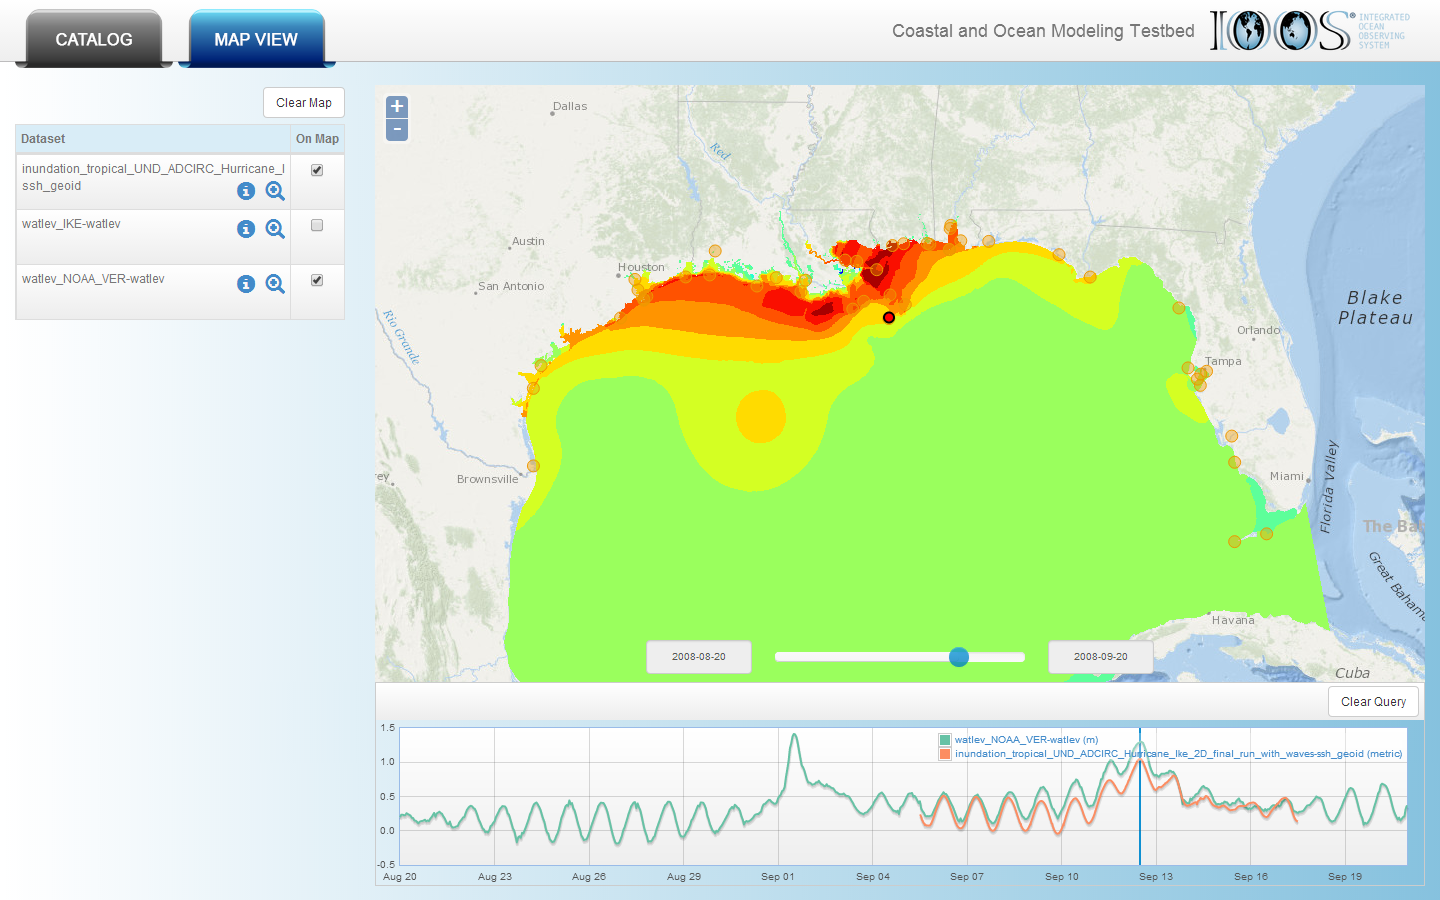
\includegraphics[width=\linewidth]{../figs/SciWMS_ModelObsComparison}
  \textbf{Figure \getIncFigcounter{}}: \textit{Comparison of ADCIRC
    (unstructured topology) model results with observed water levels
    in the Northern Gulf of Mexico for Hurricane Ike. Verified
    observed water levels are from NOAA's Station 8760922 (red dot on
    map). The map shows modeled water levels (in meters above the
    geoid) at the peak of the storm in southern Louisiana. The time
    series plot shows both the modeled (green) and observed (orange)
    water levels. The vertical blue line in the time series plot
    corresponds to the current time of the map.}
\end{minipage}

\end{document}
